\section{Induced Relational GCN}
\label{sec:gcn}
%In this section, we first summarize basic Graph convolution (GCN) model proposed for computing vertex representations in Section \ref{subsec:graph}. We then elaborate upon our operationalization of Contrastive relation in the GCN framework in Section \ref{subsec:contrast}, Similarity relation in Section \ref{subsec:similar} followed by Reflexive relation in Section \ref{subsec:reflex}.
Now, we will encode the two label assignment mechanisms within a clique
%---assign label based on the contrast with clique tuples; share labels amongst tuples in the same clique---
via a graph convolution. First, we briefly review Graph Convolution Networks (GCN) and identify some key concepts. Then, given the views $G_i$ for the four strategies, we show how to introduce label contrasts in~\Cref{subsec:contrast} followed by label sharing in~\Cref{subsec:similar}.
%We refer to the operations on each view as an Induced Relational Graph Convolutional Network (\textbf{IR-GCN}).

%This magnification results in improved separability of classes in the manifold learned by the neural network (further discussion in \cref{ref:analysis}).

\subsection{Graph Convolution}
\label{subsec:graph}
Graph Convolution models adapt the convolution operations on regular grids (like images) to irregular graph-structured data $G = (V,E)$, learning low-dimensional vertex representations. If for example, we associate a scalar with each vertex $v \in V$, where $|V| = N$, then we can describe the convolution operation on a graph by the product of signal $x \in \mathbb{R}^N$ (feature vectors) with a learned filter $g_\theta$ in the fourier domain. Thus,
\begin{equation}
  g_\theta \ast x =  U \, g_\theta \, U^T x,
  \label{eq:basic_gcn}
  % g_\theta (U \Lambda U^T) x =
\end{equation}
where, $\Lambda$ and $U$ are the eigenvalues and eigenvector of the normalized graph Laplacian, $L = I_N - D^{-\sfrac{1}{2}}AD^{\sfrac{1}{2}}$, and where $L = U \Lambda U^T$. $A$ denotes the adjacency matrix of a graph $G$ (associated with a view) with $N$ vertices. ~\Cref{eq:basic_gcn} implies a filter $g_\theta$ with $N$ free parameters, and requires expensive eigenvector decomposition of the adjacency matrix $A$. Deferrard et al.~\cite{deferrard} proposed to approximate $g_\theta$, which in general is a function of $\Lambda$, by a sum of Chebyshev polynomials $T_k(x)$ up to the $k$-th order. Then,

\begin{equation}
  g_\theta \ast x \approx U \, \sum_{k=0}^K \theta_k T_k(\tilde{\Lambda}) \, U^T x \approx \, \sum_{k=0}^K \theta_k T_k(\tilde{L}) \, x,
  \label{eq:approx_gcn}
  % g_\theta (U \Lambda U^T) x =
\end{equation}
where, $\tilde{\Lambda} = 2 \Lambda/ \lambda_{\max}- I_N$ are the scaled eigenvalues and $\tilde{L} = 2L/\lambda_{max} - I_N$ is the corresponding scaled Laplacian. Since $\tilde{L} = U \tilde{\Lambda} U^T$, the two equations are approximately equal.


%The corresponding scaled Laplacian is $\tilde{L} = 2L/\lambda_{max} - I_N$. Since $\tilde{L} = U \tilde{\Lambda} U^T$,~\Cref{eq:approx_gcn} transforms to:
% \begin{equation}
%   g_\theta \ast x \approx \, \sum_{k=0}^K \theta_k T_k(\tilde{L}) \, x.
%   \label{eq:updatedapprox_gcn}
%   % g_\theta (U \Lambda U^T) x =
% \end{equation}

The key result from Deferrard et al.~\cite{deferrard} is that~\Cref{eq:approx_gcn} implies $k$-hop localization---the convolution result depends only on the $k$-hop neighborhood. In other words,~\Cref{eq:approx_gcn}  is a $k$-hop approximation.

However, since we use equivalence relations in our framework that result in cliques, we can do an \textit{exact} convolution operation since vertices in a clique only have one-hop (i.e., $k=1$) neighbors (see lemma 5.2, \cite{Hammond2011}). The resulting convolution is linear in $L$ and now has only two filter parameters, $\theta_{0}$ and $\theta_{1}$ shared over the whole graph.
\begin{equation}
  % \begin{aligned}
g_{\theta} * x = \theta_{0}x + \theta_{1}\left(L-I_{N} \right)x %\\
  %\approx \theta_{0}x - \theta_{1}D^{-\frac{1}{2}}AD^{-\frac{1}{2}}x,
% \end{aligned}
\label{eq:restrictk}
\end{equation}

We emphasize the distinction with Kipf et al.~\cite{gcn} who approximate the Deferrard et al.~\cite{deferrard} observation by restricting $k=1$. They do so since they work on arbitrary graphs; since our relations result in views with cliques, we do not make any approximation by using $k=1$.
%We perform the convolution operation shown in~\Cref{eq:restrictk} at every layer using the outputs of the previous layer as input.





% with U denoting the eigenvector matrix of the normalized graph Laplacian $L = I_n - D^{-\sfrac{1}{2}}AD^{\sfrac{1}{2}}$ (with the decomposition $L = U \Lambda U^T$). $A$ denotes the adjacency matrix of graph $G$ with $n$ nodes (induced relational views in our case with nodes denoting $(q,a)$ tuples), $D_{ii} = \sum_j A_{ij}$ is the corresponding diagonal degree matrix.

% To circumvent the expensive eigen-decomposition of the Laplacian, \citet{deferrard} proposed to approximate $g_\theta (\Lambda)$ with truncated Chebyshev polynomials $T_k(x)$ to the $k^{th}$ order. The modified convolution is then defined as $  g_\theta * x \approx \sum_{k=0}^K \theta_k T_k(\tilde{L}) x$
%  %\begin{equation*}
% %      g_\theta * x \approx \sum_{k=0}^K \theta_k T_k(\tilde{L}) x
% % \end{equation*}
%  where $\theta \in \mathbb{R}^k$ and scaled Laplacian $\tilde{L} = 2L/\lambda_{max} - I_n$. %The Chebyshev polynomials are recursively defined as $T_k(x) = 2xT_{k-1}(x) - T_{k-2}(x)$ with $T_0(x)=1$ and $T_1(x)=x$.
%  This approximation results in spectral filters which are k-localized, i.e. they depend on the k-hop neighborhood of the node. \citet{gcn} further restricted the convolution to single-hop i.e., immediate neighborhood of the node. The resulting convolution is linear in $L$ and now has only two filter parameters, $\theta_{0}$ and $\theta_{1}$ that are shared over the whole graph.
% \begin{equation*}
%   \begin{aligned}
% g_{\theta} * x \approx \theta_{0}x + \theta_{1}\left(L-I_{n} \right)x %\\
%   %\approx \theta_{0}x - \theta_{1}D^{-\frac{1}{2}}AD^{-\frac{1}{2}}x,
% \end{aligned}
% \end{equation*}

% This can be approximated to $\theta_{0}x - \theta_{1}D^{-\sfrac{1}{2}}AD^{-\sfrac{1}{2}}x$. The authors further apply the following reduction $\theta = \theta_{0} = -\theta_{1}$.
% %\begin{equation}
% %\theta = \theta_{0} = -\theta_{1}
% %\label{hypothesis1}
% %\end{equation}
% reducing the above equation to the following additive form,
% \begin{equation}
% g_{\theta} * x \approx \theta\left(I_{n} + D^{-\sfrac{1}{2}}AD^{-\sfrac{1}{2}}\right)x,
% \end{equation}
% %Thereby, they define their model as a series of such layer wise convolutions followed by non-linear transformation of output. We use this 1-hop approximation of convolution as we deal with complete graphs.
% We can then define output of the $k^{th}$ hidden layer of graph convolution, $\mathbf{Z}^{k}$ as,
% \begin{equation}
%   \label{eq:GCN}
%   \mathbf{Z}^{k} = \sigma\left(I_N + D^{-\frac{1}{2}}AD^{\frac{1}{2}}Z^{k-1}W^{k} \right)
% \end{equation}
% $\mathbf{Z}^{k-1}$ is the output of the previous $(k-1)^{th}$ layer, and $\mathbf{Z}^{0} = X$ with the input feature matrix $X$. $\mathbb{W}^{k}$ are filter $\theta$ paramters learnt by the network; $\sigma(.)$ denotes the activation function (e.g. ReLU, tanh).

% The local graph convolution induces message-passing, with each node accumulating signals from its first-order neighborhood. In the $k^{th}$ convolutional layer, $k \in [1,\ldots,K]$, the resulting signals incorporate the $k$-hop neighborhood of each node. In each layer, the convolution %$\tilde{D}^{-\sfrac{1}{2}}\tilde{A}\tilde{D}^{\sfrac{1}{2}}$
% $I_N + {D}^{-\sfrac{1}{2}}{A}{D}^{\sfrac{1}{2}}$  in \cref{eq:GCN} results in each node's being represented by the sum of it's own features and average of it's neighborhood, followed by the linear transform $\mathbf{W}^{k}$ (see top part in ~\cref{fig:contrast}). This convolution implicitly encodes label and feature sharing across connected nodes with edges assumed to denote similarity or homogeneity between nodes.

% We now revisit the contrastive relational view, having established the message-passing nature of \cref{eq:GCN}. In the contrastive view, we aim to discriminate adjacent nodes and invert the assigned labels, i.e., capture heterogeneity in neighborhoods rather than similarity. In this setting, \cref{eq:GCN} fails to identify the contrast between the feature representations of accepted answer nodes and the rest. Thus, the vanilla GCN convolution results in misclassification of the accepted answers to the majority class of their neighborhoods. The misclassification effect is prominent in larger cliques (questions with many answers) where the neighborhood average shifts increasingly away from the features of an accepted answer. While there have been extensions of graph convolution to the inductive setting \cite{graphsage}, multi-relational setting \cite{relationalGCN}, and signed networks \cite{signedgcn}, none of these approaches are suitable to model data induced contrastive views. In the next subsection, we propose a modified convolution approach and show that it results in the form of \emph{Discriminative Feature Magnification}, highlighting feature differences between accepted answers and their neighborhoods in the contrastive views.

% %Also, note that same transformation (filter) $W^{(k)}$ is applied across all nodes in the graph.

% \begin{figure}[h]
%   \centering
% %\includegraphics[height=4cm,width=0.4\textwidth]{figures/contrast_example}\caption{\label{fig:example}Example case where original GCN framework fails.}
%   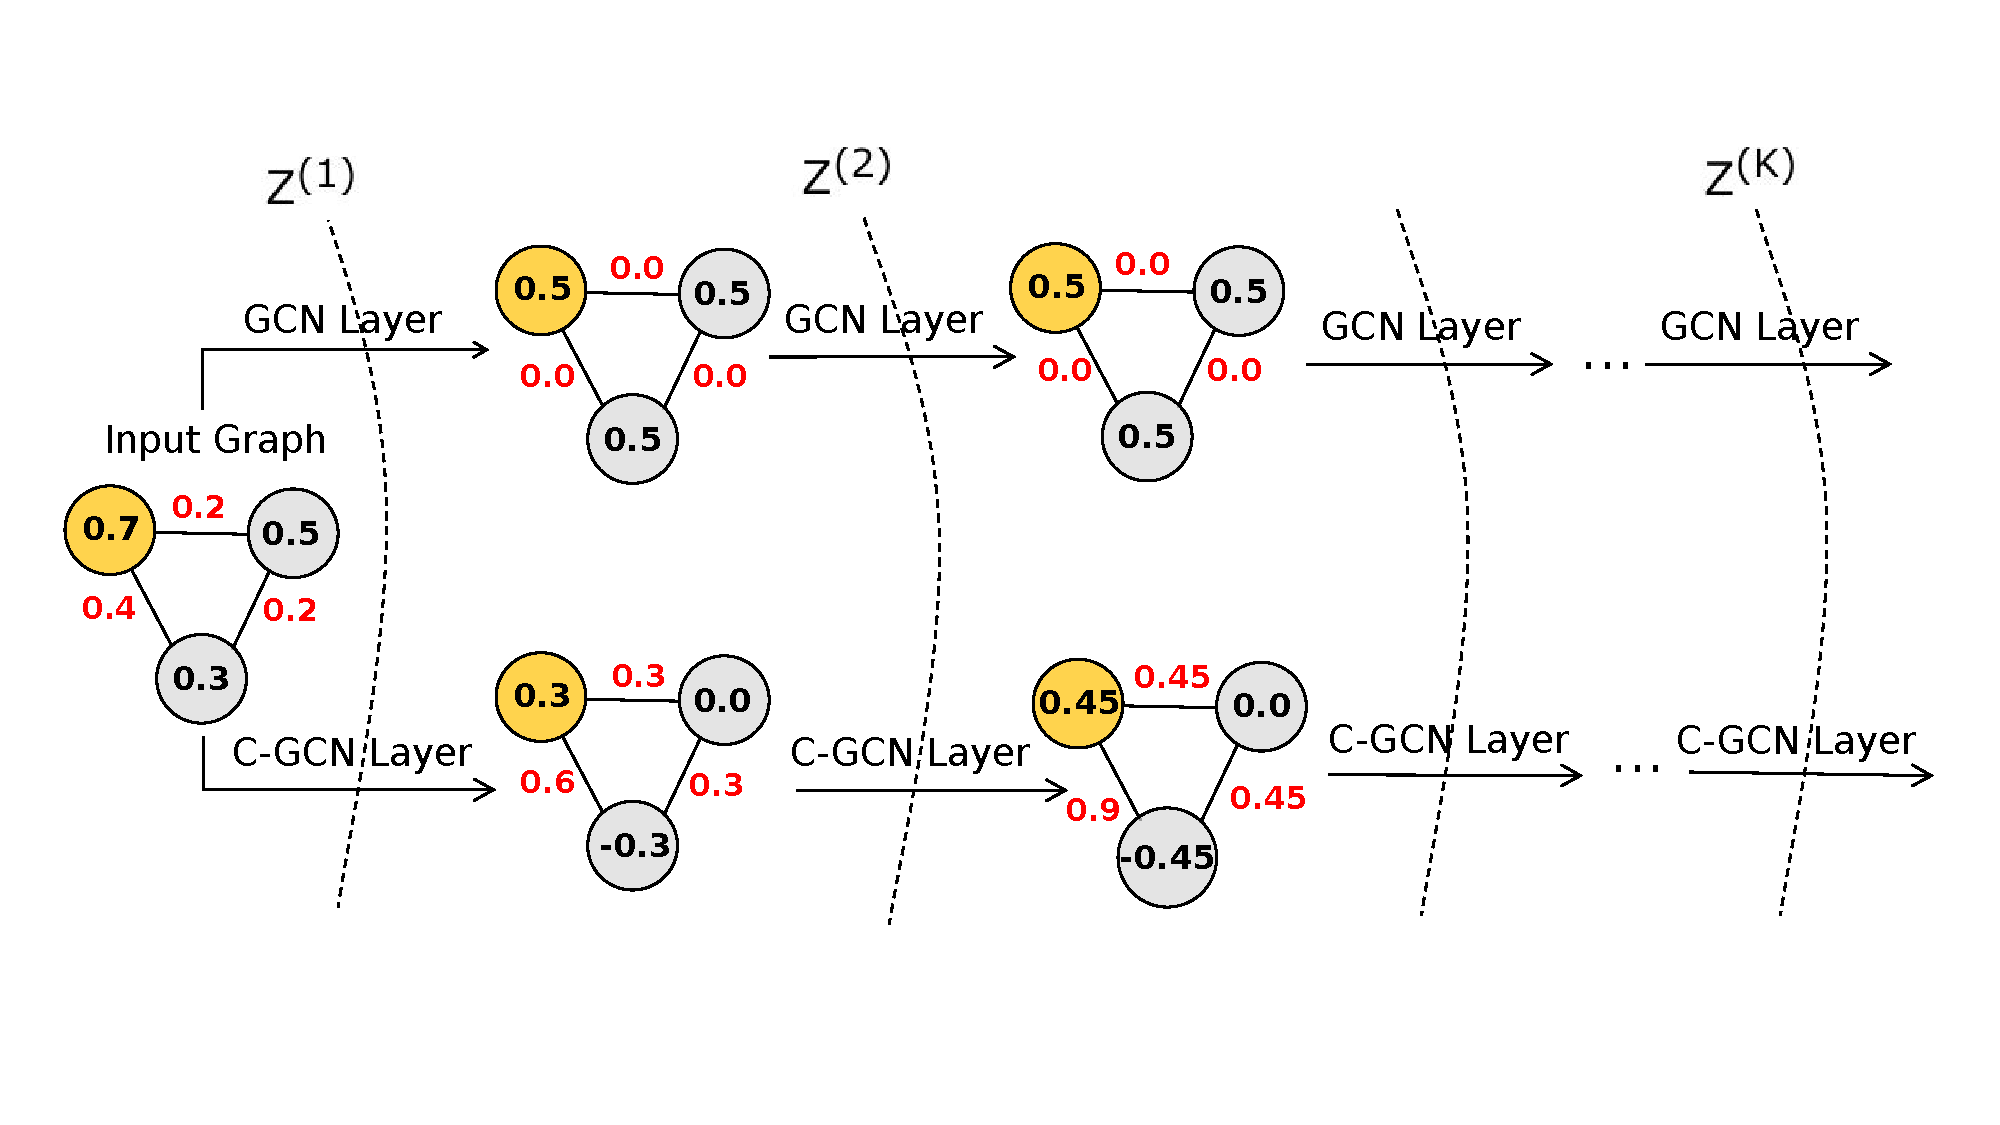
\includegraphics[scale=0.24]{figures/fig_contrast}
%   \caption{\small \label{fig:contrast}Stylized example showing the convolution results of GCN and proposed Contrastive GCN for a question with three answers. Edge labels denote the feature difference while node labels denote the resulting feature value. The feature difference between neighboring nodes increases with each convolution layer for Contrastive GCN while GCN averages the feature values among nodes. }
%     \vspace{-0.02mm}
% \end{figure}


% %For contrastive relation between, equation \ref{eq: GCN} will result in assigning feature of each answer $X_a, \forall a \in A(q)$ to question $q$, to the average of all other answers in the clique.
% %In the case of the contrastive relationship between answers, neighborhood averaging \emph{decreases} the difference between feature values of accepted and non-accepted answer and facilitates label sharing among all answers. Consider this stylized example, there are three answers $a_1$, $a_2$ and $a_3$ for question $q$ with $a_1$ being the accepted answer as shown in Figure \ref{fig:example}. Each answer has a single feature value $X$ with values being $X_{a,1} = 0.8, X_{a,2} = 0.1$ and $X_{a,3} = 0.3$. After single graph convolution operation with Identity weight matrix $W$, new feature values will be $\tilde{X}_{a,1} = \tilde{X}_{a,2} = \tilde{X}_{a,3}$ $= \sfrac{1}{3}[0.8 + 0.1 + 0.3]= 0.4$. As resulting average feature value is closer to the feature values of non-accepted class, each answer will be assigned non-accepted. This problem becomes more prominent with an increase in clique size or number of answers as neighborhood average will shift towards the non-accepted class. Note that as we are operating on a clique, subsequent graph convolutions do not change the result. Therefore, the original GCN framework is not able to identify the contrastive features of accepted answer against other non-accepted answers. This leads to misclassification of the accepted answer as the majority class of the clique, i.e., non-accepted.

% %\end{comment}

% %Most GCN based classification methods \cite{} employ a similar structure to that shown in Equation \ref{eq: GCN}, averaging of neighborhood features for each node in the graph. This approach does not work for contrastive relation setting where all neighbors need not share a class label. While there have been extensions of graph convolution to the inductive setting \cite{graphsage}, multi-relational setting \cite{relationalGCN}, and signed networks \cite{signedgcn}, none of these approaches are suitable for capturing data induced contrastive relation.

\subsection{Contrastive Graph Convolution}
\label{subsec:contrast}
% The contrastive relational view encodes contrast of each node to its neighborhood, a complementary hypothesis to the label sharing effect described in the previous section. We revisit a key simplifying assumption in \cite{gcn}, $\theta = \theta_{0} = -\theta_{1}$. This implictly encodes the similarity assumption in feature transformation.

Now, we show how to perform graph convolution to encode the mechanism of contrast, where label assignments for a tuple depend on the contrast with its neighborhood.

To establish contrast, we need to compute the \emph{difference} between the vertex's own features to its neighborhood in the clique. Thus we transform~\Cref{eq:restrictk} by setting $\theta = \theta_{0}$ = $\theta_{1}$, which essentially restricts the filters learned by the GCN. This transformation leads to the following convolution operation:
% $I_n$ and neighborhood averaged features $D^{-\frac{1}{2}}A_cD^{\frac{1}{2}}$ in the clique. We can encode this contrastive relationship by using same sign filter $\theta = \theta_{0}$ = $\theta_{1}$ which leads to this modified layer-wise convolution operation,
\begin{align}
%g_{\theta} * x &=  \theta_{0}x + \theta_{1}\left(L-I_{n} \right)x \\
g_{\theta} * x & =  \theta \left( I_N + L- I_{N} \right) x =  \theta \left( I_N - D^{-\sfrac{1}{2}} A D^{-\sfrac{1}{2}}\right) x \label{eq:contrastdetail}
% g_{\theta} * x \approx \theta\left(I_{n} - D^{-\sfrac{1}{2}}AD^{-\sfrac{1}{2}}\right)x,
\end{align}

Notice that~\Cref{eq:contrastdetail} says that for example, for any vertex $u$ with a scalar feature value $x_u$, for a given clique with $n \geq 2$ vertices, the convolution operation computes a new value $\hat{x}_u$ for vertex $u$ as follows:
\begin{equation}
  \hat{x}_u = \theta \left ( x_u - \frac{1}{n-1} \sum_{v \in \mathcal{N}_u} x_v \right ).
\end{equation}
where $\mathcal{N}_u$ is the neighborhood of vertex $u$. Notice that since our equivalence relations construct cliques, for all vertices $u$ that belong to a clique of size $n$, $|\mathcal{N}_u| = n-1$.

When we apply the convolution operation in~\Cref{eq:contrastdetail} at each layer of GCN, output for the $k$-th layer is:

% $\mathbf{Z}^{k-1}$ is the output of the previous $(k-1)^{th}$ layer, and $\mathbf{Z}^{0} = X$ with the input feature matrix $X$. $\mathbb{W}^{k}$ are filter $\theta$ paramters learnt by the network; $\sigma(.)$ denotes the activation function (e.g. ReLU, tanh).
% and the output of the $k^{th}$ convolutional layer is now given by,
\begin{equation}
  \label{eq:contrast}
  \mathbf{Z}_c^{k} = \sigma \left( \left (I_N - D^{-\sfrac{1}{2}}A_cD^{\sfrac{1}{2}} \right) \mathbf{Z}_c^{k-1} \mathbf{W}_c^{k}\right)
\end{equation}
with $A_c$ denoting the adjacency matrix in the contrastive view. $\mathbf{Z}_c^{k} \in \mathbb{R}^{N \times d}$ are the learned vertex representations for each $(q,a)$ tuple under the contrastive label assignment. $N$ is the total number of tuples and $d$ refers to the dimensionality of the embedding space. $\mathbf{Z}^{k-1}$ refers to the output of the previous $(k-1)$-{th} layer, and $\mathbf{Z}^{0} = X$ where $X$ is the input feature matrix. $\mathbf{W}_c^{k}$ are the filter $\theta$ parameters learnt by the GCN; $\sigma( \cdot)$ denotes the activation function (e.g. ReLU, $\tanh$).

% and $\mathbf{Z}_c^{k} \in \mathbb{R}^{\vert \mathcal{T} \vert \times d}$ are the learned node representations for each $(q,a)$ tuple under the contrastive strategy.

To understand the effect of~\Cref{eq:contrast} on a tuple, let us restrict our attention to a vertex $u$ in a clique of size $n$. We can do this since the convolution result in one clique is unaffected by other cliques. When we do this, we obtain:
\begin{equation}
  z_c^{k}(u) = \sigma \left(\left(z_c^{k-1}(u) - \frac{1}{n-1} \sum_{v \in \mathcal{N}_u} z_c^{k-1}(v) \right) \mathbf{W}_{c}^{k}\right). \label{eq:contrastrestrict}
  \end{equation}

% Note the effect of the change, each layer now computes the feature differences between each node and the local neighborhood, resulting in feature discrimination between contrasting nodes. Now we visit the term $(I_N - D^{-\sfrac{1}{2}}A_cD^{\sfrac{1}{2}}) \mathbf{Z}_c^{k-1}$. Under this formulation, the convolved feature value for node $i$, with neighborhood set $\mathcal{N}_i$ is given by,
% \begin{equation}
% z_c^{k}(i) = \sigma \left(\left(z_c^{k-1}(i) - \frac{1}{|\mathcal{N}_i|}\sum_{j \in \mathcal{N}_i}z_c^{k-1}(j)\right)\mathbf{W}_{c}^{k}\right)
% \end{equation}
Now consider a pair of contrasting vertices, $u$ and $v$ in the same clique of size $n$. Let us ignore the linear transform by setting $W_{c}^{k}=\mathbf{I}$ and set $\sigma(\cdot)$ to the identity function. Then we can easily verify that:

% immediate neighborhood of each other. Note that in our contrastive relational view, the nodes within each question have identical degree (say $d = |A_q|$).
\begin{equation}
z_c^{k}(u) - z_c^{k}(v) = \underbrace{
  \left (1 + \frac{1}{n-1} \right )
  }_{\text{magnification}}
  \times
  \underbrace{
    \left ( z_c^{k-1}(u) - z_c^{k-1}(v) \right )
    }_{\text{contrast in previous layer}}, \label{eq:disccontrastsimple}
\end{equation}
where, $z_c^{k}(u)$ denotes the output of the $k$-th convolution layer for the $u$-th vertex in the contrastive view. As a result, each convolutional layer magnifies the feature contrast between the vertices that belong to the same clique. Thus, the contrasting vertices move further apart. We term this as \emph{Discriminative Feature Magnification} and~\Cref{eq:disccontrastsimple} implies that we should see higher magnification effect for smaller cliques.
% An illustration is provided in the bottom part of the \cref{fig:contrast} with a uni-dimensional feature.

%Contrasting nodes are shifted further apart by \cref{eq:contrast} improving their separability in the learned manifold (further discussion in \cref{ref:analysis}).

% In our earlier example in Figure \ref{fig:example}, after applying proposed Contrastive GCN, new features values will be; $\tilde{X}_{a_1} = 0.8 - \frac{1}{2}[0.1 + 0.3] = 0.6$, $\tilde{X}_{a_2} = 0.1 - \frac{1}{2}[0.8 + 0.3] = -0.45$ and $\tilde{X}_{a_3} = 0.3 - \frac{1}{2}[0.8 + 0.1] = -0.15$.
%%For instance, in the answer selection problem, one or few of the set of answers to each question are accepted. Our objective is then to capture the contrast relation that exists between accepted answers and those that are not accepted.
%
%%\begin{comment}
%Each answer needs to \emph{contrast} between itself and rest of the answers. This can be achieved by computing the \emph{difference} instead of addition between node's own features $I_n$ and averaged features of the other nodes $D^{-\frac{1}{2}}A_cD^{\frac{1}{2}}$ in the clique. We can encode this contrastive relationship by using same sign filter $\theta = \theta_{0}$ = $\theta_{1}$ which leads to this modified layer wise convolution operation,
%\begin{equation}
%g_{\theta} * x \approx \theta\left(I_{n} - D^{-\frac{1}{2}}AD^{-\frac{1}{2}}\right)x,
%\end{equation}
%
%Thereby, output of the $k$-th hidden layer for Contrastive GCN network $Z_c^{(k)}$ is defined as:
%\begin{equation}
%  \label{eq:contrast}
%  Z_c^{(k)} = \sigma \left((I_n - D^{-\frac{1}{2}}A_cD^{\frac{1}{2}}) Z_c^{(k-1)}W_c^{(k)}\right)
%\end{equation}
%with $A_c$ as the Adjacency matrix with contrastive edges. In our earlier example in Figure \ref{fig:example}, after applying proposed Contrastive GCN, new features values will be; $\tilde{X}_{a_1} = 0.8 - \frac{1}{2}[0.1 + 0.3] = 0.6$, $\tilde{X}_{a_2} = 0.1 - \frac{1}{2}[0.8 + 0.3] = -0.45$ and $\tilde{X}_{a_3} = 0.3 - \frac{1}{2}[0.8 + 0.1] = -0.15$.
%
%\textbf{Disciminative Magnification} Note that this contrastive filter magnifies the difference between two classes, as difference between feature values, $X_{a,1}$ to $X_{a,2}$ and $X_{a,3}$ increased from $0.7$ and $0.5$ to $1.05$ and $0.75$. Stacking of this contrastive convolution layer with transformed features using $W$ weight matrix learns to magnifies the separation between features of accepted and non accepted class. This effect can be called as \emph{discriminative magnification} which improves the separation of nodes of different classes. This convolution still preserves the label sharing assumption between nodes of same class as their convolved features $\tilde{X}_{a_2} = -0.45$ and $\tilde{X}_{a_3} = -0.15$ are in similar range.

%Note that effectively the linear transformation averages the locality of a node and transforms the result linearly, layer to layer. This operation encodes an implicit notion of homophily in node classification. Nodes in similar localities or sharing neighbors are more likely to be assigned similar convolved feature representations. Alternative aggregation methods such as mean-pooling and max-pooling \cite{graphsage} achieve similar results.
%\end{comment}

 %While this does not necessarily improve the classification performance of conventional classifiers, the high VC dimension of neural networks can enable margin fitting to arbitrary regions in a high dimensional space.

%Alternately, we propose a much simpler solution to achieving node-feature contrast across convolutional layers.
%We analyze the implications of stacking the proposed convolutional contrast layers and analyze model performance in \cref{ref:analysis}.

%Also, signed edges are manually created. While graph attention networks with separate attention weight learned for each neighbor could learn negative attention weights for neighbors. However, it would be much more computationally expensive.

\subsection{Encoding Similarity Convolution}
\label{subsec:similar}
We next discuss how to encode the mechanism of sharing labels in a GCN. While label sharing applies to our similarity by contrast relation (two strategies: Arrival similarity; TrueSkill similarity, see~\Cref{sub:Induced Views}), it is also trivially applicable to the reflexive relation, where the label of the tuple only depends on itself. First, we discuss the case of similarity by contrast.

\subsubsection{Encoding Similarity by Contrast}
\label{sub:Encoding Similar Contrasts}

To encode label sharing for the two similarity by contrast cases, we transform~\Cref{eq:restrictk} with the assumption $\theta = \theta_0 = -\theta_1$. Thus

\begin{equation}
g_{\theta} * x = \theta\left(I_{N} + D^{-\sfrac{1}{2}}AD^{-\sfrac{1}{2}}\right) x, \label{eq:similargcn}
\end{equation}

%\Cref{eq:similargcn} says that for example, for any node $u$ with a scalar feature value $x_u$, for a given clique with $n\geq 2$ nodes,
Similar to the ~\Cref{eq:contrastdetail} analysis, convolution operation in \Cref{eq:similargcn} computes a new value $\hat{x}_u$ for vertex $u$ as follows:
\begin{align}
  \hat{x}_u &= \theta \left ( x_u + \frac{1}{n-1} \sum_{v \in \mathcal{N}_u} x_v \right ) = \theta \left ( \frac{n-2}{n-1} x_u + \frac{n}{n-1} \mu_x \right ).
\end{align}
That is, in the mechanism where we share labels in a clique, the convolution pushes the values of each vertex in the clique to the average feature value, $\mu_x = \frac{1}{n} \sum_{v \in \mathcal{N}_u \cup u} x_v$, in the clique.

When we apply the convolution operation in~\Cref{eq:similargcn} at each layer of GCN, output for the $k$-th layer:

% $\mathbf{Z}^{k-1}$ is the output of the previous $(k-1)^{th}$ layer, and $\mathbf{Z}^{0} = X$ with the input feature matrix $X$. $\mathbb{W}^{k}$ are filter $\theta$ paramters learnt by the network; $\sigma(.)$ denotes the activation function (e.g. ReLU, tanh).
% and the output of the $k^{th}$ convolutional layer is now given by,
\begin{equation}
  \label{eq:similar}
  \mathbf{Z}_s^{k} = \sigma \left( \left (I_N + D^{-\sfrac{1}{2}}A_sD^{\sfrac{1}{2}} \right) \mathbf{Z}_s^{k-1} \mathbf{W}_s^{k}\right)
\end{equation}
with $A_s$ denoting the adjacency matrix in the similar views.
%and $\mathbf{Z}_s^{k} \in \mathbb{R}^{N \times d}$ are the learned node representations for each $(q,a)$ tuple under the similar label assignment.
% $N$ is the total number of tuples,
% and where $d$ refers to the dimensionality of the embedding space. $\mathbf{Z}^{k-1}$ refers to the output of the previous $(k-1)$-{th} layer, and $\mathbf{Z}^{0} = X$ where $X$ is the input feature matrix. $\mathbf{W}^{k}$ are the filter $\theta$ parameters learnt by the GCN; $\sigma( \cdot)$ denotes the activation function (e.g. ReLU, $\tanh$).

We analyze the similarity GCN in a maner akin to~\Cref{eq:contrastrestrict} and
%consider a pair of similar nodes, $u$ and $v$ in the same clique of size $n$. Again, let us ignore the linear transform by setting $W_{c}^{k}=\mathbf{I}$ and set $\sigma(\cdot)$ to the identity function.Then
we can easily verify that:

% immediate neighborhood of each other. Note that in our contrastive relational view, the nodes within each question have identical degree (say $d = |A_q|$).
\begin{equation}
z_s^{k}(u) - z_s^{k}(v) = \underbrace{
  \left (1 - \frac{1}{n-1} \right )
  }_{\text{reduction}}
  \times
  \underbrace{
    \left ( z_s^{k-1}(u) - z_s^{k-1}(v) \right )
    }_{\text{contrast in previous layer}}, \label{eq:diffsimilar}
\end{equation}
where, $z_s^{k}(i)$ denotes the output of the $k$-th convolution layer for the $i$-th vertex in the similar view. As a result, each convolutional layer reduces the feature contrast between the vertices that belong to the same clique. Thus, the similar vertices move closer.

% As we observed in~\Cref{sub:Generalized Views}, three of our strategies---reflexive

% similarity relationships in the convolution framework. Recall from our discussion in ~\cref{sec:motivation}, a similarity edge connects two answers of a player if the contrast with the skill of other players answering the same question is identical. As similarity relation enforce smoothness or sharing of labels among nodes, we can directly apply the vanilla formulation (Equation \ref{eq:GCN}).
%Thus, the output of the $k$-th convolutional layer for the similarity view, $Z_s^{(k)}$ is defined as:
%\begin{equation}
%  \label{eq:similarity}
%  Z_s^{k} = \sigma \left((I_N + D^{-\frac{1}{2}}A_sD^{\frac{1}{2}}) Z_s^{(k-1)}W_s^{(k)}\right)
%\end{equation}
% However, for our experiments, we report better results without using renormalization trick.
%In this section, we showed how to encode the similarity mechanism where we share labels amongst vertices that belong to the same clique.

The proposed label sharing encoding applies to both similarity by contrast strategies (TrueSkill; Arrival). We refer to the corresponding vertex representations as $\mathbf{Z}_{ts}^{k}$ (TrueSkill), $\mathbf{Z}_{as}^{k}$ (Arrival).

%Recall from our discussed in Section \ref{sec:motivation}, a similarity edge connects two answers of a player if the contrast with the skill of other players answering the same question is identical. This follows from the principle that if there is a top ranked player, even if other players in the game have decent rankings, he would outplay all of them. In such scenarios, such contrastive answers from the top ranked player ought to share label and thus form a clique. Similar argument follows for the opposite case when you are outranked by all players in the game. We operationalize contrastive similarity using two data induced relationships.

%\textbf{True Skill Similarity} connects answers of the same answerer where difference in skill value of the answerer with other answerers for a question has a significant margin $\delta$. We estimate user's skill value using TrueSkill rating system \cite{TrueSkill06} computed on the basis of accepted label of user's all answers in the community.
%
%% developed by Microsoft Reasearch for ranking and matching similar skill game players for Xbox Live. In our settings, each question is a multi player game with all answerers as game players. The user who gives credible answer is the winner. True Skill rating then computes player's skill through bayesian inference on the basis of credibility label of his answered questions. The estimated ratings are a Gaussian distribution where $\mu$ denotes the average skill of the player. We use the mean value as skill value for our computations.
%
%Therefore, each user can have at most two cliques, one which connects all his answers where his true skill is significantly better than other answerers of the question; and second where his skill is vastly lower than all the other answerers. In the first case, he is highly likely to give accepted answers while in other, his answer would be classified as non-accepted. As CQA platforms encompass variety of topics, each user can be accepted in one topic while non accepted for other topics in the same community. \\MARGIN?
%Formally, output of the $k$-th hidden layer for True Skill Similarity GCN network $Z_{ts}^{(k)}$ is defined as:
%\begin{equation}
%  \label{eq:TSsimilarity}
%  Z_{ts}^{k} = \sigma\left((I_N + D^{-\frac{1}{2}}A_{ts}D^{\frac{1}{2}}) Z_{ts}^{(k-1)}W_s^{(k)} \right)
%\end{equation}
%with $A_{ts}$ being the adjacency matrix for true skill similarity relations.
%
%

%Thus, for each user, we construct a clique of all answers in which he answers significantly earlier than other answers, and another clique with all answers in which his answer is much later than all other answers for that question. Formally, output of the $k$-th hidden layer for Arrival Similarity GCN network $Z_{as}^{(k)}$ is defined as:
%\begin{equation}
%  \label{eq:ASsimilarity}
%   Z_{as}^{k} = \sigma \left((I_N + D^{-\frac{1}{2}}A_{as}D^{\frac{1}{2}}) Z_{as}^{(k-1)}W_s^{(k)} \right)
%\end{equation}
%with $A_{as}$ being the adjacency matrix for arrival similarity relationship.

\subsubsection{Reflexive Convolution}
\label{subsubsec:reflex}
We encode the reflexive relation with self-loops in the graph resulting in an identity adjacency matrix. This relation is the trivial label sharing case, with an independent assignment of vertex labels. Thus, the output of the $k$-th convolutional layer for the reflexive view, $\mathbf{Z}_r^{k}$ reduces to:
\begin{equation}
  \label{eq:reflexive}
  \mathbf{Z}_r^{k} = \sigma \left( I_N \mathbf{Z}_r^{k-1} \mathbf{W}_r^{k} \right)
\end{equation}
Hence, the reflexive convolution operation is equivalent to a feedforward neural network with multiple layers and activation $\sigma( \cdot )$.

\vspace{0.1in}
\noindent
%Each strategy $i \in \mathbf{S}$ produces a view $G_i = (V, E_i)$ with identical vertex set $V$.
Each strategy $S_i \in \mathbf{S}$ belongs to one of the three relation types---reflexive, contrastive and similarity, where $\mathbf{R}$ denotes the set of strategies of that relation type. $\mathcal{R} = \bigcup \mathbf{R}$ denotes the set of all relation types.
%We apply all strategies on each vertex $v \in V$ corresponding to tuple $(q,a)$.
%We combine the results of the embeddings from the each of the four strategies as follows. Let $v \in V$ correspond to the tuple $(q,a)$.
$\mathbf{Z}_i^K \in \mathbb{R}^{N X d}$ represents the $d$ dimensional vertex embeddings for strategy $S_i$ at the $K$-th layer. For each strategy $S_i$, we obtain a scalar score by multiplying $\mathbf{Z}_i^K$ with transform parameters $\widetilde{W}_i \in \mathbb{R}^{d \times 1}$.
%Each strategy $\mathbf{S}_k$ produces a view $G_i = (V, E_i)$ with identical vertex set $V$. We apply each of the $i=4$ strategies $\mathbf{S}_k \in \mathcal{S}$ on each vertex $v \in V$ corresponding to tuple $(q,a)$. We combine the results of the embeddings from the each of the four strategies as follows. Let $v \in V$ correspond to the tuple $(q,a)$. Let $\mathbf{Z}_i^K(v)$ be the the $d$ dimensional embedding for node $v$, strategy $i$ at the $K$-th layer. For each strategy $i$, we project $\mathbf{Z}_i^K(v)$ to a scalar using transform parameters $\widetilde{W}_i \in \mathbb{R}^{d \times 1}$.
%Thus, for each relation type $\mathbf{R} \in \mathcal{R}$, and their corresponding views $i \in \mathbf{R}$, their convolution generates node representations $\mathbf{Z}_{i}^{K} \in \mathbb{R}^{N \times d}$ for each node $v \in V$. Each $Z_{i}^{K}$ is projected to generate a single score or prediction outcome for that view using transform parameters $\widetilde{W}_i \in \mathbb{R}^{d \times 1}$.
The sum of these scores gives the combined prediction score, $\mathbf{H}_{\mathbf{R}} \in \mathbb{R}^{N X 1}$, for that relation type.
%of all strategies, $S_i \in \mathbf{R}$.
%relation type $\mathbf{R}$ for each node over the graph convolutions with the different views $G_i , \forall i \in \mathbf{R}$ of that relation type,
\begin{equation}
    \label{eq:score}
        \mathbf{H}_{\mathbf{R}} = \sum_{S_i \in \mathbf{R}} \mathbf{Z}_i^K \widetilde{W}_i^T
\end{equation}

%The induced views under \emph{Similarity by contrast} strategy semantically differ from the view under \emph{Contrastive} strategy in two ways. First, they enable feature sharing between the connected nodes. In the \emph{Contrastive} strategy, the objective is feature discrimination; a node that contrasts with its neighbors is likely to have a different label. These semantics are captured in the convolutional architecture we apply to those views (\cref{subsec:contrast}, \cref{subsec:similar}). Second, since there are multiple ways to construct \emph{Similarity by contrast} views, they depend on the similarity measure (TrueSkill and Arrival Similarity are two relevant metrics in CQA). Views within a strategy are likely to be correlated. Our architecture combines cross-strategy and intra-strategy views appropriately to encode this difference (\cref{sec:aggregation}).

In this section, we proposed Graph Convolutional architectures to compute vertex representations of each $(q,a)$ tuple under the four strategies. %Each strategy induces cliques and used one of three relationship types---\textit{contrastive}, \textit{similar contrast} and \textit{reflexive}.
%Each strategy induces cliques, and within a clique
In particular, we showed how to encode two different label assignment mechanisms---label sharing and determine label based on contrast---within a clique. The architecture that encodes label assignment based on contrast is a novel contribution, distinct from the formulations presented by Kipf et al.~\cite{gcn} and its extensions~\cite{signedgcn,relationalGCN}. Prior convolutional architectures implicitly encode the label sharing mechanism (~\cref{eq:similargcn}); however, label sharing is unsuitable for contrastive relationships across vertices. Hence our architecture fills this gap in prior work.

%Now, we proceed to develop and compare aggregation approaches to combine the predictions of the different strategies.
%\clearpage
